%% Time-stamp: <2018-10-18 20:24:12 (marc)>
\documentclass[xcolor=x11names,compress, mathserif]{beamer}

\newcommand{\hackspace}{\hspace{4.2mm}}
\newcommand{\showstudent}[1]{}
\newcommand\hmmax{0}
\newcommand\bmmax{0}





% talk/author information
\newcommand{\authorname}{Yingzhen Li}
\newcommand{\authoremail}{yingzhen.li@imperial.ac.uk}
\newcommand{\authortwitter}{liyzhen2}
\newcommand{\authoraffiliation}{
  Department of Computing\\Imperial
  College London}
\newcommand{\slidesettitle}{\imperialBlue{Principal Component Analysis}}
\newcommand{\footertitle}{Principal Component Analysis (PCA)}
\newcommand{\location}{Imperial College London}
\newcommand{\talkDate}{Nov 21, 2022}



\date{\imperialGray{\talkDate}}




% load defaults
%\usepackage{../MarkMathCmds}
\input{../includes/header.tex}
\input{../includes/YingzhenNotations.tex}



\input{../includes/titlepage.tex}
\linespread{1.2}


\begin{frame}{Dimensionality reduction}

\begin{minipage}{0.8\linewidth}
High-dimensional raw data are often sparse, \\perhaps lying on a low-dimensional manifold:
\end{minipage}
\hfill
\begin{minipage}{0.15\linewidth}
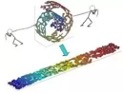
\includegraphics[width=1\linewidth]{figures-pca/dim_reduction_vis1.jpg}
\end{minipage}

\begin{figure}
\centering
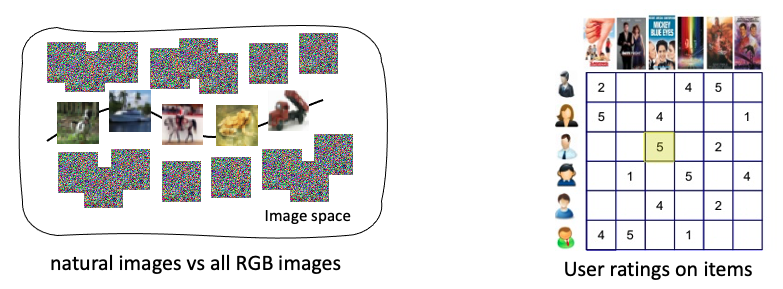
\includegraphics[width=0.9\linewidth]{figures-pca/dim_reduction_vis2.png}
\end{figure}

\end{frame}


\begin{frame}{Dimensionality reduction}
To name a few dimensionality reduction methods:

\begin{figure}
\centering
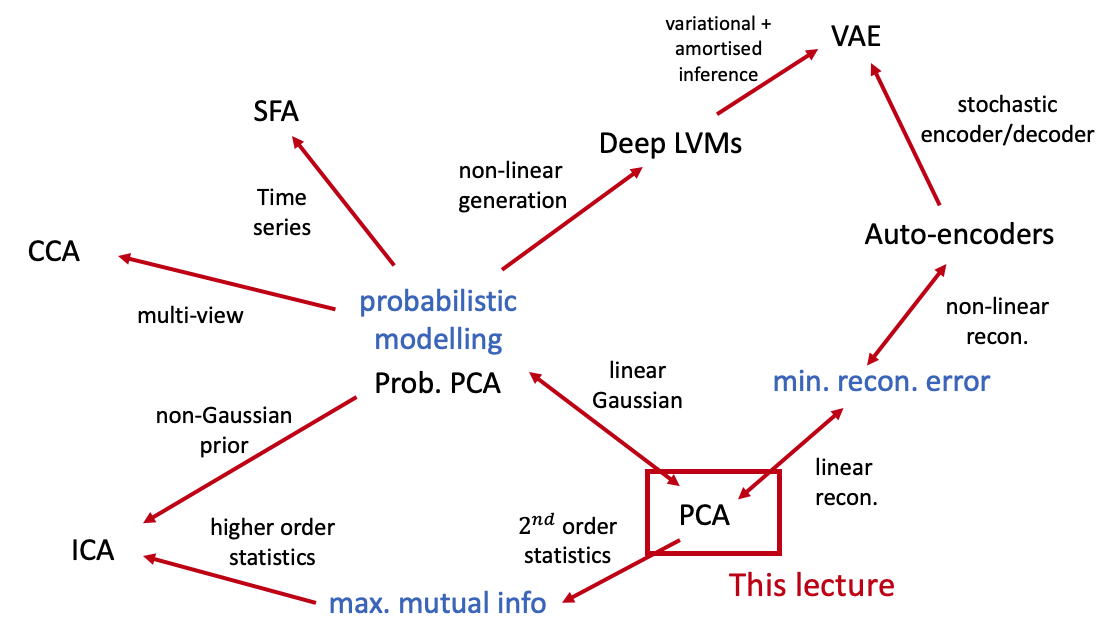
\includegraphics[width=0.9\linewidth]{figures-pca/dim_reduction_methods_vis2.png}
\end{figure}

\end{frame}

\begin{frame}{PCA in practise}

\begin{figure}
\centering
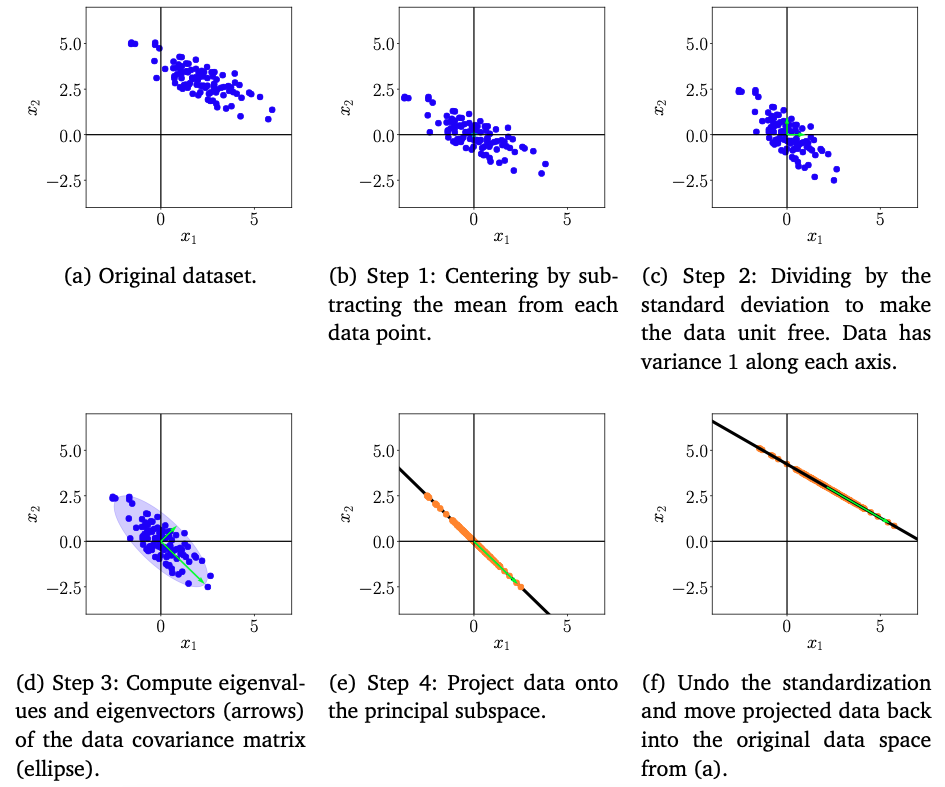
\includegraphics[width=0.7\linewidth]{figures-pca/keysteps_pca.png}
\end{figure}
\hfill \tiny{Fig from the MML book.}

\end{frame}



\begin{frame}{PCA: set-up}
Problem set-up:
\begin{itemize}
\item Data: $\data = \{\x_1, ..., \x_N \}$, $\x_n \in \mathbb{R}^{D\times 1}$ s.t. $\text{mean}(\x_n) = \bm{0}$
\item Find projections in a \alert{lower-dimensional} space: 
$$\x_n \approx \tilde{\x}_n := \sum_{j=1}^{\textcolor{red}{M}} \z_{nj} \Bb_j, \quad \z_{nj} := \Bb^\top_j \x_n$$
using an \alert{orthonormal basis}
$$\BB = [\Bb_1, ..., \Bb_M], \quad \Bb_m \in \mathbb{R}^{D \times 1}, \quad \textcolor{red}{M < D}$$
\end{itemize}

\end{frame}


\begin{frame}{Quick refresher: basis}

For a given datapoint $\x_n = [\x_{n1}, ..., \x_{nD}]^\top \in \mathbb{R}^{D\times 1}$

\begin{figure}
\centering
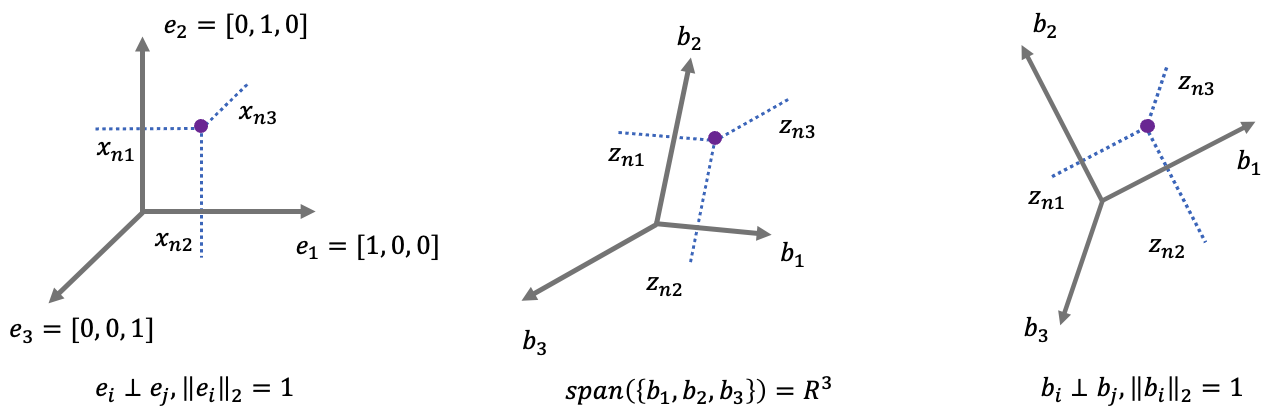
\includegraphics[width=1\linewidth]{figures-pca/basis_visual.png}
\end{figure}
\vspace{-1em}
\hfill \footnotesize{$\uparrow$ orthonormal basis}

Coordinates $\{ \z_{nj} \}$ are projections of the $\x_n$ vector onto a given basis:
$$\x_n = \sum_{j=1}^D \z_{nj} \Bb_j, \quad \z_{nj} := \Bb_j^\top \x_n$$
\end{frame}


%%%%%%%%%%%%%%%%%%%%%%
\begin{frame}{PCA: maximum variance perspective}

The ``maximum variance'' intuition of PCA:

project onto directions where the datapoints ``vary the most''

\begin{minipage}{0.5\linewidth}
\only<1>{
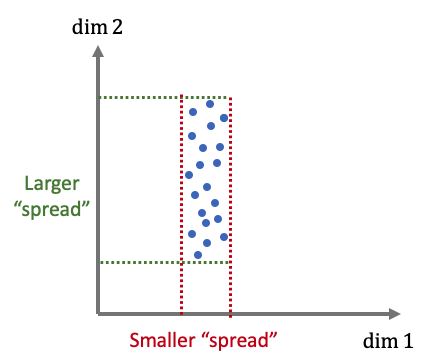
\includegraphics[width=0.8\linewidth]{figures-pca/pca_variance_intuition1.png}
}
\only<2->{
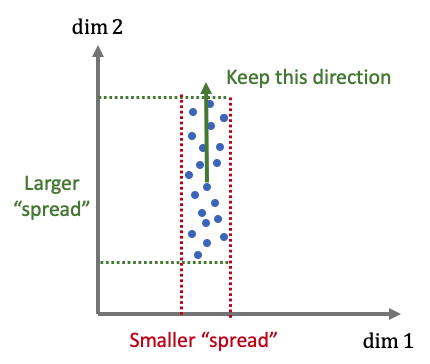
\includegraphics[width=0.8\linewidth]{figures-pca/pca_variance_intuition2.png}
}
\end{minipage}
\hfill
\begin{minipage}{0.45\linewidth}
\only<3>{
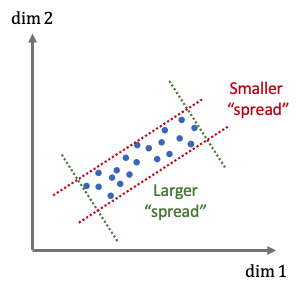
\includegraphics[width=0.8\linewidth]{figures-pca/pca_variance_intuition3.png}
}
\only<4>{
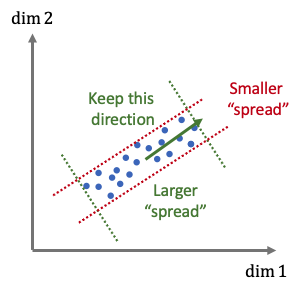
\includegraphics[width=0.8\linewidth]{figures-pca/pca_variance_intuition4.png}
}
\end{minipage}
\vspace{1em}

``Spread'' is defined as the variance along a given direction

\end{frame}

\begin{frame}{PCA: maximum variance perspective}
Problem set-up:
\begin{itemize}
\item Data: $\data = \{\x_1, ..., \x_N \}$, $\x_n \in \mathbb{R}^{D\times 1}$ s.t. $\text{mean}(\x_n) = \bm{0}$
\item Find projections in a \alert{lower-dimensional} space: 
$$\z_n := \BB^\top \x_n  \quad \Leftrightarrow \quad \z_{nj} := \Bb^\top_j \x_n $$
using an \alert{orthonormal basis}
$$\BB = [\Bb_1, ..., \Bb_M], \quad \Bb_m \in \mathbb{R}^{D \times 1}, \quad \textcolor{red}{M < D}$$
\item Solve for $\Bb_1$ such that
$$ \mathbb{V}[\Bb_1^\top \x_n] \quad \text{is maximised}$$
\end{itemize}

\end{frame}

\begin{frame}{PCA: maximum variance perspective}
Solve for $\Bb_1$ such that
$$ \mathbb{V}[\Bb_1^\top \x_n] \quad \text{is maximised,    subject to } || \Bb_1 ||_2 = 1$$

\vspace{-0.5em}
\begin{itemize}
\item Variance after projection (recall that $\x_n$ has mean zero): 
\begin{equation*}
\begin{aligned}
\mathbb{V}[\Bb_1^\top \x_n] &:= \frac{1}{N} \sum_{n=1}^N (\Bb_1^\top \x_n)^2 = \Bb_1^\top (\textcolor{red}{\underbrace{\frac{1}{N}\sum_{n=1}^N \x_n \x_n^\top}_{:=\BS = \BQ \Lambda \BQ^\top }} ) \Bb_1 \\
&= \Bb_1^\top \BQ \Lambda \underbrace{\BQ^\top \Bb_1}_{:= \bm{\beta}_1} = \sum_{d=1}^D \lambda_d \beta_{1d}^2
\end{aligned}
\end{equation*}

\item $|| \Bb_1 ||_2^2 = 1 \quad \Rightarrow \quad || \bm{\beta}_1 ||_2^2 = 1$ 
\begin{equation*}
|| \Bb_1 ||_2^2 := \Bb_1^\top \Bb_1 = \Bb_1^\top \textcolor{red}{\underbrace{\BQ \BQ^\top}_{=\mathbf{I}}} \Bb_1 = (\BQ^\top \Bb_1 )^\top (\underbrace{\BQ^\top \Bb_1}_{:= \bm{\beta}_1} ) =  \bm{\beta}_j^\top \bm{\beta}_j = || \bm{\beta}_1 ||_2^2
\end{equation*}

\end{itemize}

\end{frame}

\begin{frame}{PCA: maximum variance perspective}
Solve for $\Bb_1$ such that
$$ \mathbb{V}[\Bb_1^\top \x_n] \quad \text{is maximised,    subject to } || \Bb_1 ||_2 = 1$$

\begin{itemize}
\item Equivalent to solving the following problem 
$$ \max_{\bm{\beta}_1} \sum_{d=1}^D \lambda_d \beta_{1d}^2 \quad \text{ s.t.} || \bm{\beta}_1 ||_2^2 = \sum_{d=1}^D \beta_{1d}^2 = 1.$$


\item \alert{Solution: $\bm{\beta}_1 = \bm{e}_1 := (1, 0, ..., 0)^\top$} \\ $\Rightarrow \Bb_1 = \bm{q}_1$ (the eigenvector with the largest eigenvalue)
\end{itemize}

\end{frame}


\begin{frame}{PCA: maximum variance perspective}
Iteratively solve for the rest of the directions $\Bb_2, ... \Bb_M$:

For $m = 2, ..., M$: 
\begin{itemize}
\item Compute the ``remainder'' of projection: 
$$\textcolor{red}{\hat{\x}_n} = \x_n - \sum_{j=1}^{m-1} \z_{nj} \Bb_j = \x_n - \sum_{j=1}^{m-1} (\Bb_j^\top \x_n) \Bb_j$$ \pause

\item maximise the following objective w.r.t.~$\Bb_m$: 
$$\max_{\Bb_m} \mathbb{V}[\Bb_m^\top \textcolor{red}{\hat{\x}_n}], \quad \text{s.t. } || \Bb_m ||_2 = 1, \Bb_m \perp \Bb_j, j = 1, ..., m-1$$
\end{itemize}

\end{frame}

\begin{frame}{PCA: maximum variance perspective}
Iteratively solve for the rest of the directions $\Bb_2, ... \Bb_M$:

For $m = 2, ..., M$: 

\begin{itemize}
\item maximise $\mathbb{V}[\Bb_m^\top \hat{\x}_n]$, subject to $|| \Bb_m ||_2 = 1$, $\Bb_m \perp \Bb_j, j = 1, ..., m-1$

\item Recall that $\x_n$ has mean zero:
\begin{equation*}
\begin{aligned}
\mathbb{V}[\Bb_m^\top \hat{\x}_n] &:= \frac{1}{N} \sum_{n=1}^N (\Bb_m^\top \x_n - \sum_{j=1}^{m-1} (\Bb_j^\top \x_n) \textcolor{red}{\underbrace{\Bb_j^\top \Bb_m}_{=0}})^2 = \Bb_m^\top (\textcolor{red}{ \underbrace{\frac{1}{N} \sum_{n=1}^N \x_n \x_n^\top}_{=\BS = \BQ \Lambda \BQ^\top}} ) \Bb_m \\
&= \Bb_m^\top \BQ \Lambda \underbrace{\BQ^\top \Bb_m}_{:= \bm{\beta}_m} = \sum_{d=1}^D \lambda_d \beta_{md}^2
\end{aligned}
\end{equation*}

\item Here $\Lambda = diag(\lambda_1, ..., \lambda_d)$ and $\lambda_1 \geq ... \geq \lambda_D \geq 0$.

\end{itemize}

\end{frame}


\begin{frame}{PCA: maximum variance perspective}
Iteratively solve for the rest of the directions $\Bb_2, ... \Bb_M$:

For $m = 2, ..., M$: 
\begin{itemize}
\item maximise $\mathbb{V}[\Bb_m^\top \hat{\x}_n]$, subject to $|| \Bb_m ||_2 = 1$, $\Bb_m \perp \Bb_j, j = 1, ..., m-1$

\item $|| \Bb_m ||_2^2 = 1 \quad \Rightarrow \quad || \bm{\beta}_m ||_2^2 = 1$ 
\begin{equation*}
\hspace{-1em}
|| \Bb_m ||_2^2 := \Bb_m^\top \Bb_m = \Bb_m^\top \textcolor{red}{\underbrace{\BQ \BQ^\top}_{=\mathbf{I}}} \Bb_m = (\BQ^\top \Bb_m )^\top (\underbrace{\BQ^\top \Bb_m}_{:= \bm{\beta}_m} ) =  \bm{\beta}_m^\top \bm{\beta}_m = || \bm{\beta}_m ||_2^2
\end{equation*}

\item $\Bb_m \perp \Bb_j \quad \Rightarrow \quad \Bb_m^\top \Bb_j = 0 \quad \Rightarrow \quad \bm{\beta}_m^\top \bm{\beta}_j = 0$
\begin{equation*}
\Bb_m^\top \Bb_j = \Bb_m^\top \textcolor{red}{\underbrace{\BQ \BQ^\top}_{=\mathbf{I}}} \Bb_j = (\underbrace{\BQ^\top \Bb_m}_{:= \bm{\beta}_m} )^\top (\underbrace{\BQ^\top \Bb_j}_{:= \bm{\beta}_j} ) =  \bm{\beta}_m^\top \bm{\beta}_j 
\end{equation*}

\end{itemize}
\end{frame}



\begin{frame}{PCA: maximum variance perspective}
Iteratively solve for the rest of the directions $\Bb_2, ... \Bb_M$:

For $m = 2, ..., M$:
\begin{itemize}
\item maximise $\mathbb{V}[\Bb_m^\top \x_n]$, subject to $|| \Bb_m ||_2 = 1$, $\Bb_m \perp \Bb_j, j = 1, ..., m-1$

\item Equivalent to the following optimisation problem:
$$ \max_{\bm{\beta}_m} \sum_{d=1}^D \lambda_d \beta_{md}^2 \quad \text{ s.t.} || \bm{\beta}_m ||_2^2 =1, \bm{\beta}_m^\top \bm{\beta}_j = 0, j = 1, ..., m-1.$$
\end{itemize}

Proof by induction: we show $\bm{\beta}_m = \bm{e}_m := (0, ..., 0, \underbrace{1}_{m\text{th element}}, 0, ..., 0)$

\vspace{-0.5em}
\begin{itemize}
\item[1.] $\bm{\beta}_1 = \bm{e}_1 \quad \Rightarrow \quad \Bb_1 = \bm{q}_1$ \pause
\item[2.] For $m=2, ..., M$, assume $\bm{\beta}_j = \bm{e}_j, j = 1, ..., m-1$
\begin{itemize}
	\item[2a.] $\bm{\beta}_m^\top \bm{\beta}_j = 0, j = 1, ..., m-1 \quad \Rightarrow \quad \bm{\beta}_{mj} = 0, j = 1, ..., m-1$ \pause
	\item[2b.] $||\bm{\beta}_m ||_2 = 1 \quad \Rightarrow \quad \sum_{d=m}^D \beta_{md}^2 = 1$ \pause
	\item[2c.] Solve for maximum of $\sum_{d=m}^D \lambda_d \beta_{md}^2$ w.r.t.~$\beta_{md}$:
	\\ \alert{Solution: $\bm{\beta}_m = \bm{e}_m \quad \Rightarrow \quad \Bb_m = \bm{q}_m$}
\end{itemize}
\end{itemize}

\end{frame}


\begin{frame}{PCA: maximum variance perspective}

For $m = 1, ..., M$:
\begin{itemize}
\item maximise $\mathbb{V}[\Bb_m^\top \x_n]$, subject to $|| \Bb_m ||_2 = 1$, $\Bb_m \perp \Bb_j, j = 1, ..., m-1$
\end{itemize}

\alert{Solutions:} $\Bb_m = \bm{q}_m$ for $m = 1, ..., M$

$\Rightarrow$ Projecting $\x_n$ to a subspace 
$$span(\{ \bm{q}_m \}_{m=1}^M) = span(\{ \bm{q}_j \}_{j=M+1}^D)^{\perp}$$

\vspace{-1em}
\begin{minipage}{0.7\linewidth}
\begin{equation*}
\x_n = \textcolor{blue}{\underbrace{\sum_{j=1}^M \z_{nj} \bm{q}_j }_{:= \tilde{\x}_n}} + \textcolor{red}{\underbrace{\sum_{j=M+1}^D \z_{nj} \Bb_j}_{\text{dropped}}}, \quad \Bb_i \perp \bm{q}_j
\end{equation*}
$$\tilde{\x}_n \in span(\{ \bm{q}_m \}_{m=1}^M)$$
\end{minipage}
\hfill
\begin{minipage}{0.25\linewidth}
\centering
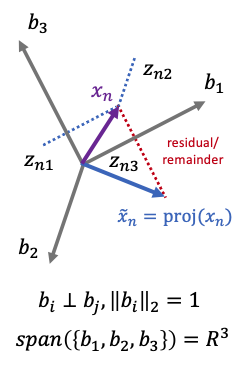
\includegraphics[width=0.9\linewidth]{figures-pca/pca_recon_intuition2.png}
\end{minipage}

\end{frame}


%%%% PCA: minimum error view

\begin{frame}{PCA: minimum reconstruction error perspective}

Goal: find orthonormal basis $\{\Bb_1, ..., \Bb_M \}$ to minimise $\ell_2$ reconstruction error:
\begin{equation*}
L = \frac{1}{N} \sum_{n=1}^N || \x_n - \tilde{\x}_n ||_2^2, \quad \tilde{\x}_n := \sum_{j=1}^M \z_{nj} \Bb_j, \ \z_{nj} = \Bb_j^\top \x_n.
\end{equation*}

Rewriting the loss:

\begin{minipage}{0.7\linewidth}

\begin{itemize}
\item Consider the full orthonormal basis:
$$\BB_{full} = [ \underbrace{\Bb_1, ..., \Bb_M}_{\text{will be used in new basis}}, \underbrace{\Bb_{M+1}, ..., \Bb_{D}}_{\text{will be dropped}}]$$
\vspace{-1em}
\item Representing $\x_n$ using basis $\BB_{full}$:
\end{itemize}
\only<1>{
\begin{equation*}
\x_n = \textcolor{blue}{\underbrace{\sum_{j=1}^M \z_{nj} \Bb_j }_{:= \tilde{\x}_n} } + \textcolor{red}{ \sum_{j=M+1}^D \z_{nj} \Bb_j}, \quad \z_{nj} := \Bb^\top_j \x_n
\end{equation*}
}
\only<2>{
\begin{equation*}
\x_n - \textcolor{blue}{\tilde{\x}_n} = \textcolor{red}{ \sum_{j=M+1}^D \z_{nj} \Bb_j}, \quad \z_{nj} := \Bb^\top_j \x_n
\end{equation*}
}

\end{minipage}
\hfill
\begin{minipage}{0.25\linewidth}

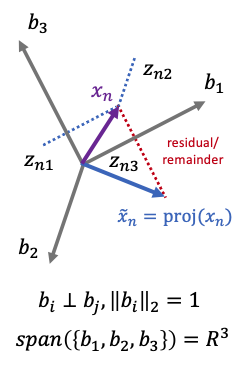
\includegraphics[width=1\linewidth]{figures-pca/pca_recon_intuition2.png}

\end{minipage}

\end{frame}

\begin{frame}{PCA: minimum reconstruction error perspective}

Goal: find orthonormal basis $\{\Bb_1, ..., \Bb_M \}$ to minimise $\ell_2$ reconstruction error:
\begin{equation*}
L = \frac{1}{N} \sum_{n=1}^N || \x_n - \tilde{\x}_n ||_2^2, \quad \tilde{\x}_n := \sum_{j=1}^M \z_{nj} \Bb_j, \ \z_{nj} = \Bb_j^\top \x_n.
\end{equation*}

Rewriting the loss:

\only<1>{
First notice that $\BB_{full}$ is an \alert{orthonormal} basis:
\begin{equation*}
\begin{aligned}
L &= \frac{1}{N} \sum_{n=1}^N || \sum_{j=M+1}^D \z_{nj} \Bb_j ||_2^2 \\
&= \frac{1}{N} \sum_{n=1}^N \sum_{j=M+1}^D || \z_{nj} \Bb_j ||_2^2 \\
&= \frac{1}{N} \sum_{n=1}^N \sum_{j=M+1}^D \z_{nj}^2
\end{aligned}
\end{equation*}
}

\only<2>{
Plugging-in that $\z_{nj} = \Bb_j^\top \x_n$:
\begin{equation*}
\begin{aligned}
L &= \frac{1}{N} \sum_{n=1}^N \sum_{j=M+1}^D (\Bb_j^\top \x_n)^2 = \frac{1}{N} \sum_{n=1}^N \sum_{j=M+1}^D \Bb_j^\top (\x_n \x_n^\top) \Bb_j \\
&= \sum_{j=M+1}^D \Bb_j^\top ( \textcolor{red}{\underbrace{\frac{1}{N} \sum_{n=1}^N \x_n \x_n^\top}_{:=\BS = \BQ \Lambda \BQ}}) \Bb_j = \sum_{j=M+1}^D \Bb_j^\top \BQ \Lambda \underbrace{\BQ^\top \Bb_j}_{:= \bm{\beta}_j} = \sum_{j=M+1}^D \sum_{d=1}^D \lambda_d \beta_{jd}^2
\end{aligned}
\end{equation*}
}

\end{frame}


\begin{frame}{PCA: minimum reconstruction error perspective}

Assume the eigenvalue decomposition as $\BS = \BQ \Lambda \BQ^\top$, \\
with $\Lambda = diag([\lambda_1, ..., \lambda_D]), \lambda_1 \geq \cdots \geq \lambda_D$
\begin{equation*}
\begin{aligned}
\Bb_j^\top \BS \Bb_j &= \Bb_j^\top \BQ \Lambda \BQ^\top \Bb_j := \bm{\beta}_j^\top \Lambda \bm{\beta}_j = \sum_{d=1}^D \lambda_d \beta_{jd}^2 \\
\bm{\beta}_j &:= \BQ^\top \Bb_j = [\beta_{j1}, ..., \beta_{jD}] = [\bm{q}_1^\top \Bb_j, ..., \bm{q}_D^\top \Bb_j]
\end{aligned}
\end{equation*}

\begin{itemize}
\item $|| \Bb_j ||_2^2 = 1 \quad \Rightarrow \quad || \bm{\beta}_j ||_2^2 = 1$ 
\begin{equation*}
|| \Bb_j ||_2^2 := \Bb_j^\top \Bb_j = \Bb_j^\top \textcolor{red}{\underbrace{\BQ \BQ^\top}_{=\mathbf{I}}} \Bb_j = (\BQ^\top \Bb_j )^\top (\underbrace{\BQ^\top \Bb_j}_{:= \bm{\beta}_j} ) =  \bm{\beta}_j^\top \bm{\beta}_j = || \bm{\beta}_j ||_2^2
\end{equation*}

\item $\Bb_i \perp \Bb_j \quad \Rightarrow \quad \Bb_i^\top \Bb_j = 0 \quad \Rightarrow \quad \bm{\beta}_i^\top \bm{\beta}_j = 0$
\begin{equation*}
\Bb_i^\top \Bb_j = \Bb_i^\top \textcolor{red}{\underbrace{\BQ \BQ^\top}_{=\mathbf{I}}} \Bb_j = (\underbrace{\BQ^\top \Bb_i}_{:= \bm{\beta}_i} )^\top (\underbrace{\BQ^\top \Bb_j}_{:= \bm{\beta}_j} ) =  \bm{\beta}_i^\top \bm{\beta}_j 
\end{equation*}

\end{itemize}

\end{frame}


\begin{frame}{PCA: minimum reconstruction error perspective}

\begin{equation*}
\text{min}_{\bm{\beta}_{M+1:D}} \ L  = \sum_{j=M+1}^D \sum_{d=1}^D \lambda_d \beta_{jd}^2, \quad \text{s.t.} \ || \bm{\beta}_j ||_2^2 = 1, \ \bm{\beta}_i^\top \bm{\beta}_j = 0.
\end{equation*}

An iterative approach for solutions: \\
Solve $\bm{\beta}_D$ first and then solve for $\bm{\beta}_j$ for $j = D - 1, ..., M+1$. 

\begin{itemize}
\item Optimisation objective for $\bm{\beta}_D$:
$$\text{min}_{\bm{\beta}_D} \sum_{d=1}^D \lambda_d \beta_{Dd}^2, \quad \text{s.t.} \ || \bm{\beta}_D ||_2^2 = \sum_{d=1}^D \beta_{Dd}^2 = 1 $$ 
\item Notice: $\lambda_1 \geq \cdots \geq \lambda_D$ 
\item \alert{Solution}: $\bm{\beta}_D = \bm{e}_D := (0, ..., 0, 1)^\top$ \\ 
$\Rightarrow \ \Bb_D = \bm{q}_D$ (the eigenvector with the smallest eigenvalue)
\end{itemize}

\end{frame}

\begin{frame}{PCA: minimum reconstruction error perspective}

\begin{equation*}
\text{min}_{\bm{\beta}_{M+1:D}} \ L  = \sum_{j=M+1}^D \sum_{d=1}^D \lambda_d \beta_{jd}^2, \quad \text{s.t.} \ || \bm{\beta}_j ||_2^2 = 1, \ \bm{\beta}_i^\top \bm{\beta}_j = 0.
\end{equation*}

Proof by induction: for $j = D, D - 1, ..., M+1$, $\bm{\beta}_j = \bm{e}_j$, i.e., $\Bb_j = \bm{q}_j$
 
\begin{itemize}
\item[1.] For $j = D$: $\bm{\beta}_D = \bm{e}_D$, i.e., $\Bb_D = \bm{q}_D$ 
\item[2.] For $j = D-1, ..., M+1$, assume for $i > j$, $\bm{\beta}_i = \bm{e}_i$, i.e., $\Bb_i = \bm{q}_i$ 

\begin{itemize}
	\item[2a.] $\bm{\beta}_i^\top \bm{\beta}_j = 0, i > j \quad \Rightarrow \quad \bm{\beta}_j = (\beta_{j1}, ..., \beta_{jj}, 0, ..., 0)^\top$ \pause
	\item[2b.] $||\bm{\beta}_j ||^2_2 = 1 \quad \Rightarrow \quad \sum_{d=1}^j \beta_{jd}^2 = 1$ \pause
	\item[2c.] Solve for the following minimisation problem w.r.t.~$\beta_{jd}$:
	\only<4>{
	$$\text{min}_{\bm{\beta}_j} \sum_{d=1}^j \lambda_d \beta_{jd}^2, \quad \text{s.t.} \ \sum_{d=1}^j \beta_{jd}^2 = 1 $$
	}
	\only<5->{
	\\ \alert{Solution: $\bm{\beta}_j = \bm{e}_j$, i.e., $\Bb_j = \bm{q}_j$ }
	}
\end{itemize}
\end{itemize}

\end{frame}

\begin{frame}{PCA: minimum reconstruction error perspective}

\vspace{-1em}
\begin{equation*}
\begin{aligned}
\text{min}_{\BB_{full}} \ L  = \frac{1}{N} \sum_{n=1}^N || \x_n - \tilde{\x}_n ||_2^2, \quad \tilde{\x}_n := \sum_{j=1}^M \z_{nj} \Bb_j \\ 
\text{s.t.} \ || \Bb_j ||_2^2 = 1, \Bb_i \perp \Bb_j
\end{aligned}
\end{equation*}

\alert{Solutions:} $\Bb_j = \bm{q}_j$ for $j = M+1, ..., D$

$\Rightarrow$ Projecting $\x_n$ to an orthogonal complement space 
$$span(\{ \bm{q}_j \}_{j=M+1}^D)^{\textcolor{red}{\perp}} = \{ \x \in \mathbb{R}^{D\times 1}: \x^\top \bm{q}_j = 0, j = M+1, ..., D \}$$

\vspace{-1em}
\begin{minipage}{0.7\linewidth}
\begin{equation*}
\x_n = \textcolor{blue}{\underbrace{\sum_{j=1}^M \z_{nj} \Bb_j }_{:= \tilde{\x}_n}} + \textcolor{red}{\underbrace{\sum_{j=M+1}^D \z_{nj} \bm{q}_j}_{\text{dropped}}}, \quad \Bb_i \perp \bm{q}_j
\end{equation*}
$$\tilde{\x}_n \in span(\{ \bm{q}_j \}_{j=M+1}^D)^{\textcolor{red}{\perp}}$$
\end{minipage}
\hfill
\begin{minipage}{0.25\linewidth}
\centering
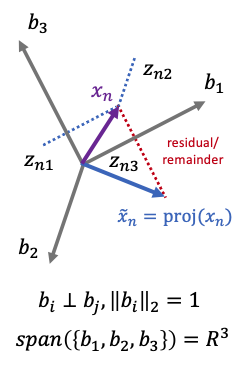
\includegraphics[width=0.9\linewidth]{figures-pca/pca_recon_intuition2.png}
\end{minipage}

\end{frame}

%%%%%%%%

\begin{frame}{PCA: comparing both views}
\begin{itemize}
%
\item Maximum variance view:
$$\BB_{full}^* = \{ \bm{q}_1, ..., \bm{q}_M, \Bb_{M+1}, ..., \Bb_D \}, \quad \Bb_i \perp \Bb_j, \Bb_i \perp \bm{q}_j$$ 

\item Minimum reconstruction error view:
$$\BB_{full}^* = \{ \Bb_1, ..., \Bb_M, \bm{q}_{M+1}, ..., \bm{q}_D \}, \quad \Bb_i \perp \Bb_j, \Bb_i \perp \bm{q}_j$$

\item No unique solution! By convention we often use $\BB_{full}^* = \BQ$

\item Relates to the equivalence between PCA and \emph{linear auto-encoder} \\ (exercise for you)
\end{itemize}

\end{frame}

%%%%%%%





\end{document}
%%% Local Variables: 
%%% mode: latex
%%% TeX-master: t
%%% End: 
